%-----------------------------------------------------------------------
% Beginning of chap2.tex
%-----------------------------------------------------------------------
%
%  AMS-LaTeX sample file for a chapter of a monograph, to be used with
%  an AMS monograph document class.  This is a data file input by
%  chapter.tex.
%
%  Use this file as a model for a chapter; DO NOT START BY removing its
%  contents and filling in your own text.
% 
%%%%%%%%%%%%%%%%%%%%%%%%%%%%%%%%%%%%%%%%%%%%%%%%%%%%%%%%%%%%%%%%%%%%%%%%


\chapter*{Lecture 8}
\addcontentsline{toc}{chapter}{Lecture 8}
\addtocounter{chapter}{8}
\addtocounter{section}{0}
%\numberwithin{section}{chapter}
\numberwithin{equation}{chapter}
\numberwithin{theorem}{chapter}

% \epigraph{}{--- \textup{}}

Linear programming is about problems of the form
\begin{align*}
 \maximize & \ip{\vct{c}}{\vct{x}}\\
 \subjto & \mtx{A}\vct{x}\leq \vct{b},
\end{align*}
where $\mtx{A}\in \R^{m\times n}$, $\vct{x}\in \R^n$, $\vct{c}\in \R^n$, and $\vct{b}\in \R^m$, and the inequality sign means inequality in each row. The {\em feasible set} is the set of all possible candidates, 
\begin{equation*}
 \mathcal{F} = \{\vct{x}\in \R^n \mid \mtx{A}\vct{x}\leq \vct{b}\}.
\end{equation*}
This set can be empty (example: $x\leq 1, \ -x\leq -2$), unbounded (example: $x\leq 1$) or bounded (example: $x\leq 1$, $-x\leq 0$). In any case, it is a convex set. To understand linear programming it is of paramount importance to understand the geometry of the feasible sets of linear programming, also called {\em polyhedra}.

\section{Linear Programming Duality: a first glance}
Suppose we are faced with a linear programming problem and would like to know if the feasible set $\mathcal{F}$ is empty or not, i.e., if $\mtx{A}\vct{x}\leq \vct{b}$ has a solution. If it is not empty, we can certify that by producing a vector from $\mathcal{F}$. To verify that the feasible set is empty is more tricky: we are asked to show that {\em no} vector lives in $\mathcal{F}$. What we can try to do, however, is to show that the assumption of a solution to $\mtx{A}\vct{x}\leq \vct{b}$ would lead to a contradiction.
Denote by $\vct{a}_i^{\trans}$ the rows of $\mtx{A}$. Assuming $\vct{x}\in \mathcal{F}$, then given a vector $\zerovct\neq \vct{\lambda}=(\lambda_1,\dots,\lambda_m)^{\trans}$ with $\lambda_i\geq 0$, the linear combination satisfies
\begin{equation}\label{eq:lincomb}
 \sum_{i=1}^m\lambda_i \vct{a}_i^{\trans}\vct{x} \leq \sum_{i=1}^m \lambda_i b_i = \ip{\vct{\lambda}}{\vct{b}}.
\end{equation}
If we can find parameters $\vct{\lambda}$ such that the left-hand side of~\eqref{eq:lincomb} is identically $0$ and the right-hand side is strictly negative, then we have found a contradition and can conclude that no $\vct{x}$ satisfies $\mtx{A}\vct{x}\leq \vct{b}$. A condition that ensures this is
\begin{equation}\label{eq:dual}
 \sum_{i=1}^m \lambda_i\vct{a}_i = \zerovct, \quad \ip{\vct{\lambda}}{\vct{b}} < 0.
\end{equation}
In matrix form,
\begin{equation*}
 \exists \vct{\lambda}\geq \zerovct, \ \mtx{A}^{\trans}\vct{\lambda}=\zerovct, \ \ip{\vct{\lambda}}{\vct{b}}<0.
\end{equation*}
This condition will still be satisfied if we normalise the vector $\vct{\lambda}$ such that $\sum_{i=1}^m\lambda_i=1$, so the statement says that $\zerovct$ is a convex combination of the vectors defining the equations.

\begin{example}Consider the system
\begin{align}\label{eq:ex1}
\begin{split}
 x_1+x_2 &\leq 2\\
 -x_1 &\leq -1\\
 -x_2 &\leq -1.5.
 \end{split}
\end{align}
The transpose matrix $\mtx{A}^{\trans}$ and the vector $\vct{b}$ are
\begin{equation*}
 \mtx{A}^{\trans} = \begin{pmatrix}
                     1 & -1 & 0 \\
                     1 & 0 & -1 
                    \end{pmatrix}, \quad
 \vct{b} = \begin{pmatrix}
            2 \\ -1 \\ -1.5.
           \end{pmatrix}
\end{equation*}
Drawing the columns of $\mtx{A}^{\trans}$ we get
\begin{figure}[h!]
\centering
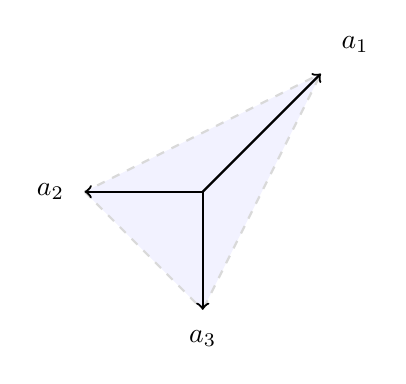
\begin{tikzpicture}[thick,scale=1.5]
\draw[color=black!15, fill=blue!5, thick, rounded corners=2pt, dashed] (-1,0)--(0,-1)--(1,1)--(-1,0);
\node (A1) at (1,1)  [label=45:{$\vct{a}_1$}] {};
\node (A2) at (-1,0)  [label=180:{$\vct{a}_2$}] {};
\node (A3) at (0,-1)  [label=270:{$\vct{a}_3$}] {};
\draw[color=black,->] (0,0)--(1,1);
\draw[color=black,->] (0,0)--(0,-1);
\draw[color=black,->] (0,0)--(-1,0);

\end{tikzpicture}
\end{figure}
We can get the origin as a convex combination of the vectors $\vct{a}_i$ (drawing a rope around them encloses the origin), and such a combination is given by $\vct{\lambda}=(1/3,1/3,1/3)$. Taking the scalar product with the vector $\vct{b}$ we get
\begin{equation*}
 \ip{\vct{\lambda}}{\vct{b}} = \frac{1}{3}(2-1-1.5) = -\frac{1}{6}<0.
\end{equation*}
This shows that the system~\eqref{eq:ex1} does not have a solution (a fact that in this simple example can also be seen by drawing a picture).
\end{example}

It turns out that Condition~\eqref{eq:dual} is not only sufficient but also necessary, and the separating hyperplane theorem is an essential part of this. We first make a detour in order to better understand the feasible sets, the polyhedra.

\section{Polyhedra}

\begin{definition}
 A polyhedron (plural: polyhedra) is a set defined as the solution of linear equalities and inequalities,
 \begin{equation}\label{eq:polyhedron}
  P = \{\vct{x}\in \R^d \mid \mtx{A}\vct{x}\leq \vct{b}\},
 \end{equation}
where $\mtx{A}\in \R^{m\times d}$, $\vct{b}\in \R^m$. 
\end{definition}

More classically, we can write out the equations.
\begin{align}\label{eq:eq}
\begin{split}
 a_{11}x_1+\cdots +a_{1d}x_d &\leq b_1,\\
 \cdots& \\
 a_{m1}x_1+\cdots +a_{md}x_d & \leq b_m.
 \end{split}
\end{align}

We now introduce some useful terminology and concepts associated to polyhedra, and illustrate them with a few examples.
A supporting hyperplane $H$ of a polyhedron $P$ is a hyperplane such that $P\subseteq H_-$, where $H_-$ is a halfspace associated to $H$. If $H$ is a supporting hyperplane, then a set of the form $F=H\cap P$ is called a {\em face} of $P$. In particular, the polyhedron $P$ is a face.
Each of the inequalities $\ip{\vct{a}_i}{\vct{x}}\leq b_i$ in~\eqref{eq:polyhedron} defines a supporting hyperplane, and therefore a face. The {\em dimension} of a face $F$,
$\dim F$, is the smallest dimension of an affine space containing $F$. Faces of dimension $\dim F=\dim P-1$ are called {\em facets}, faces of dimension $0$ are vertices, and of dimension $1$ edges. A vertex can equivalently be characterised as a point $\vct{x}\in P$ that can not be written as a convex combination of two other points in $P$.

\begin{example}
 Polyhedra in one dimension are the sets $[a,b]$, $[a,\infty)$, $(-\infty,b]$, $\R$ or $\emptyset$, where $a\leq b$. Each of them is clearly convex.
\end{example}

\begin{example}\label{ex:trian}
 The set
 \begin{equation*}
  P=\{\vct{x}\in \R^2 \mid x_1+x_2\leq 1, \ x_1\geq 0, \ x_2\geq 0\}.
 \end{equation*}
is the polyhedron shown in Figure~\ref{fig:triangle}. We can write the defining inequalities in standard form $\mtx{A}\vct{x}\leq \vct{b}$ by setting 
\begin{equation*}
 \mtx{A} = \begin{pmatrix}
            1 & 1\\
            -1 & 0\\
            0 & -1
           \end{pmatrix}, \quad
 \vct{b} = \begin{pmatrix}
            1 \\ 0 \\ 0
           \end{pmatrix}.
\end{equation*}
\begin{figure}[h!]
\centering
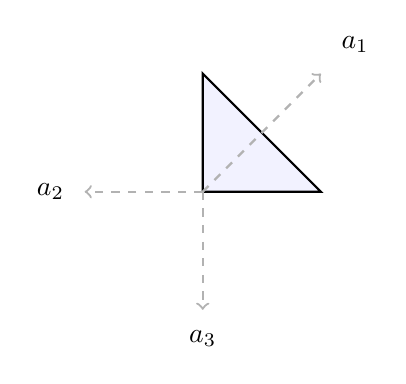
\begin{tikzpicture}[thick,scale=1.5]
\node (A1) at (1,1)  [label=45:{$\vct{a}_1$}] {};
\node (A2) at (-1,0)  [label=180:{$\vct{a}_2$}] {};
\node (A3) at (0,-1)  [label=270:{$\vct{a}_3$}] {};
\draw[fill=blue!5] (-0,0)--(0,1)--(1,0)--(0,0);
\draw[dashed,color=black!30,->] (0,0)--(1,1);
\draw[dashed,color=black!30,->] (0,0)--(0,-1);
\draw[dashed,color=black!30,->] (0,0)--(-1,0);
\end{tikzpicture}
\caption{A two-dimensional polyhedron and defining equations.}\label{fig:triangle}
\end{figure}
This polyhedron has one face of dimension $2$ (itself), three facets of dimension $1$ (the sides, corresponding to the three equations), and three vertices of dimension $0$ (the corners, corresponding any two of the defining equations).
\end{example}

\begin{example}\label{ex:durer}
 The polyhedron in Albrecht D\"urer's famous ``Melencolia I'', aka the ``truncated triangular trapezohedron'', can be described using eight inequalities, see Figure~\ref{fig:melen}.
 
 \begin{figure}[h!]
 \centering
 \begin{minipage}{0.5\textwidth}
 \centering
  \includegraphics[width=0.8\textwidth]{images/melancolia.jpg}
 \end{minipage}%
 \begin{minipage}{0.45\textwidth}
\begin{align*}
    0.7071x_1   -0.4082x_2 +  0.3773x_3 & \leq 1\\
   -0.7071x_1 +   0.4082x_2  -0.3773x_3 & \leq 1\\
    0.7071x_1 +   0.4082x_2  -0.3773x_3 & \leq 1\\
   -0.7071x_1   -0.4082x_2 +  0.3773x_3 & \leq 1\\
                  0.8165x_2 +  0.3773x_3 & \leq 1\\
                 -0.8165x_2  -0.3773x_3 & \leq 1\\
                               0.6313x_3 & \leq 1\\
                              -0.6313x_3 & \leq 1
\end{align*}
\end{minipage}
\caption{D\"urer's Melencolia and equations defining the polyhedron}\label{fig:melen}
\end{figure}
% can be described by the equations $\mtx{A}\vct{x}\leq \vct{b}$, where
% \begin{equation*}
% \mtx{A} = \begin{pmatrix}
%   0.7071 &   -0.4082 &   0.3773\\
%    -0.7071 &   0.4082 &  -0.3773\\
%     0.7071 &   0.4082 &  -0.3773\\
%    -0.7071 &  -0.4082 &   0.3773\\
%          0 &   0.8165 &   0.3773\\
%          0 &  -0.8165 &  -0.3773\\
%          0 &        0 &   0.6313\\
%          0 &        0 &  -0.6313
%          \end{pmatrix}, \quad
%          \vct{b}=\begin{pmatrix}
%                   1\\1\\1\\1\\1\\1\\1\\1
%                  \end{pmatrix}.
% \end{equation*}
\end{example}

We now move to a different characterization of bounded polyhedra. The main result of this lecture is that bounded polytopes can be described completely from knowing their vertices. A polyhedron $P$ is called bounded, if there exists a ball $B(\zerovct,r)$ with $r>0$ such that $P\subset B(\zerovct,r)$. For example, halfspaces are not bounded, but the polytope from Examples~\ref{ex:trian} and~\ref{ex:durer} are.

We first observe the nontrivial fact that a polyhedron has only fin

\begin{definition}
 A {\em polytope} is the convex hull of finitely many points,
 \begin{equation*}
  P = \conv(\{x_1,\dots,x_k\}) = \{\sum_{i=1}^k \lambda_i\vct{x}_i, \ \lambda_i\geq 0, \sum_i \lambda_i=1\}.
 \end{equation*}
\end{definition}

\begin{theorem}\label{thm:main1}
 A bounded polyhedron $P$ is the convex hull of its vertices.
\end{theorem}

\begin{example}
The triangle in Example~\ref{ex:trian} is the convex hull of the points $(0,0)^{\trans}$, $(0,1)^{\trans}$, and $(1,0)^{\trans}$.
\end{example}

\begin{example}
 The D\"urer polytope is the convex hull of the following 12 vertices:
 \begin{align*}
  \vct{v}_1 &= \begin{pmatrix} -1.4142\\   -0.8165\\   -0.8835 \end{pmatrix},
   \vct{v}_2 = \begin{pmatrix}-1.4142\\    0.8165\\    0.8835 \end{pmatrix}, 
   \vct{v}_3 = \begin{pmatrix}-0.8536\\   -0.4928\\   -1.5840 \end{pmatrix}, 
   \vct{v}_4 = \begin{pmatrix}-0.8536\\    0.4928\\    1.5840 \end{pmatrix}, \\
   \vct{v}_5 &= \begin{pmatrix}-0.0000\\   -1.6330\\    0.8835 \end{pmatrix}, 
   \vct{v}_6 = \begin{pmatrix} 0.0000\\   -0.9856\\    1.5840 \end{pmatrix}, 
   \vct{v}_7 = \begin{pmatrix}-0.0000\\    0.9856\\   -1.5840 \end{pmatrix}, 
   \vct{v}_8 = \begin{pmatrix} 0.0000\\    1.6330\\   -0.8835 \end{pmatrix}, \\ 
   \vct{v}_9 &= \begin{pmatrix}0.8536\\   -0.4928\\   -1.5840 \end{pmatrix}, 
   \vct{v}_{10} = \begin{pmatrix} 0.8536\\    0.4928\\    1.5840 \end{pmatrix}, 
   \vct{v}_{11} = \begin{pmatrix} 1.4142\\   -0.8165\\   -0.8835 \end{pmatrix}, 
   \vct{v}_{12} = \begin{pmatrix} 1.4142\\    0.8165\\    0.8835 \end{pmatrix}. 
 \end{align*}

\end{example}

The converse of Theorem~\ref{thm:main1} is also true.

\begin{theorem}
 A polytope is a bounded polyhedron.
\end{theorem}

The equivalence between polytopes and bounded polyhedra gives a first glimpse into linear programming duality theory, a topic of central importance in both modeling and algorithm design.



% %-----------------------------------------------------------------------
% % End of chap1.tex
% %-----------------------------------------------------------------------
